\documentclass{article}

%%%%%%%%%%%%%%%%%%%%%%%%%%%%%%%%%%%%%%%%%%%%%%%%%%%%%%%%%%%%%%%%%
%package

%geometry
\usepackage[a4paper]{geometry}%调整页面边距
\geometry{left=3cm,right=3cm,top=2.5cm,bottom=3cm}
\linespread{1.5}
\usepackage{fancyhdr}%梦幻页眉

%fonts
\usepackage{fontspec}%字体库
\defaultfontfeatures{Mapping=tex-text}
\usepackage{xunicode,xltxtra}
\usepackage[BoldFont,SlantFont,CJKnumber,CJKchecksingle]{xeCJK}  % \CJKnumber{12345}: 一万二千三百四十五
\usepackage{CJKfntef}
\usepackage{bm} %公式中的粗体字符\boldsymbol
\usepackage{pifont}

%color
\usepackage{color,xcolor}
\definecolor{GREEN}{RGB}{25,180,68}
\definecolor{YELLOW}{RGB}{255,255,224}
\definecolor{BLUE}{RGB}{9,148,234}
\definecolor{RED}{RGB}{139,0,0}
\definecolor{DRED}{RGB}{128,0,0}
\definecolor{GREY}{RGB}{128,128,128}
\usepackage[pagecolor={YELLOW}]{pagecolor}%设置页面底色

%math
\usepackage{amsmath,amsfonts,amssymb}

%graphics
\usepackage[americaninductors,europeanresistors]{circuitikz}
\usepackage{tikz}%可以绘制各种坐标图,方格图
\usetikzlibrary{positioning,arrows,shadows,shapes,calc,mindmap,trees,backgrounds}  % placements=positioning
\usepackage{graphicx}%\includegraphics插图命令
\usepackage{subfigure}  %%图形或表格并排排列

% table
\usepackage{colortbl,dcolumn}  %% 彩色表格
\usepackage{multirow}
\usepackage{multicol}
\usepackage{booktabs}

% code
\usepackage{fancyvrb}%漂亮的代码包
\usepackage{listings}%加入代码

% ref
\usepackage{hyperref}%扩展参考文献,目录功能和加入超链接。

% title
\usepackage{titlesec}%花哨的章节标题

\usepackage{etoolbox}
\makeatletter
\patchcmd{\ttlh@hang}{\parindent\z@}{\parindent\z@\leavevmode}{}{}
\patchcmd{\ttlh@hang}{\noindent}{}{}{}
\makeatother%titlesec旧版本无编号问题


\titleformat
{\section} % command
[display] % shape
{\bfseries\Large} % format
{第\ \thesection 章\ } % label
{0.3ex} % sep
{
    \rule{\textwidth}{1pt}
    \vspace{1ex}
    \centering
} % before-code
[
\vspace{-2ex}%
\rule{\textwidth}{1pt}
] % after-code


%tightly-packed lists
\usepackage{mdwlist}
\usepackage{verbatim}%comment命令的注释包
\usepackage{styles/zhfontcfg}%中文包
\usepackage{styles/iplouclistings}
\usepackage{styles/iplouccfg}

% head/foot
\setlength{\headheight}{15pt}
\pagestyle{fancy}
\fancyhf{}



%%%%%%%%%%%%%%%%%%%%%%%%%%%%%%%%%%%%%%%%%%%%%%%%%%%%%%%%%%%%%%%%%%%%%%

%settings
\setCJKmainfont{Adobe Kaiti Std} %设置为楷体
\setCJKmonofont{Adobe Fangsong Std}%仿宋
%页眉页脚


\makeatletter
\def\headrule{{\if@fancyplain\let\headrulewidth\plainheadrulewidth\fi%
\hrule\@height 2.5pt \@width\headwidth\vskip1pt%上面线为2.5pt粗  
\hrule\@height 0.5pt\@width\headwidth  %下面0.5pt粗            
\vskip-2\headrulewidth\vskip-1pt}      %两条线的距离        
\vspace{16mm}}     %双线与下面正文之间的垂直间距              
\makeatother         
                       
\chead{\color{GREY}LATEX-GETTINGSTARTED}%页眉
\cfoot{\color{GREY}Augeust 2016}%页脚 中
\lfoot{\color{GREY}Dinghao}%页脚 左
\rfoot{\color{GREY}$\cdot$\ Page \thepage\ }%页脚 右
\renewcommand{\headrulewidth}{0.4pt}
\renewcommand{\footrulewidth}{0.4pt}


% graphics
\graphicspath{{figures/}}
\tikzset{
    % Define standard arrow tip
    >=stealth',
    % Define style for boxes
    punkt/.style={
           rectangle,
           rounded corners,
           draw=black, very thick,
           text width=6.5em,
           minimum height=2em,
           text centered},
    % Define arrow style
    pil/.style={
           ->,
           thick,
           shorten <=2pt,
           shorten >=2pt,},
    % Define style for FlyZhyBall
    FlyZhyBall/.style={
      circle,
      minimum size=6mm,
      inner sep=0.5pt,
      ball color=red!50!blue,
      text=white,},
    % Define style for FlyZhyRectangle
    FlyZhyRectangle/.style={
      rectangle,
      rounded corners,
      minimum size=6mm,
      ball color=red!50!blue,
      text=white,},
    % Define style for zhyfly
    zhyfly/.style={
      rectangle,
      rounded corners,
      minimum size=6mm,
      ball color=red!25!blue,
      text=white,},
    % Define style for new rectangle
    nrectangle/.style={
      rectangle,
      draw=#1!50,
      fill=#1!20,
      minimum size=5mm,
      inner sep=0.1pt,}
}

% code
\lstnewenvironment{VHDLcode}[1][]{%
  \lstset{
    basicstyle=\footnotesize\ttfamily\color{black},%
    columns=flexible,%
    framexleftmargin=.7mm,frame=shadowbox,%
    rulesepcolor=\color{blue},%
%    frame=single,%
    backgroundcolor=\color{yellow!20},%
    xleftmargin=1.2\fboxsep,%
    xrightmargin=.7\fboxsep,%
    numberstyle=\tiny\color{blue},%
    numberblanklines=false,numbersep=7pt,%
    language=VHDL%
    }\lstset{#1}}{}
\lstnewenvironment{VHDLmiddle}[1][]{%
  \lstset{
    basicstyle=\scriptsize\ttfamily\color{black},%
    columns=flexible,%
    framexleftmargin=.7mm,frame=shadowbox,%
    rulesepcolor=\color{blue},%
%    frame=single,%
    backgroundcolor=\color{yellow!20},%
    xleftmargin=1.2\fboxsep,%
    xrightmargin=.7\fboxsep,%
    numbers=left,numberstyle=\tiny\color{blue},%
    numberblanklines=false,numbersep=7pt,%
    language=VHDL%
    }\lstset{#1}}{}
\lstnewenvironment{VHDLsmall}[1][]{%
  \lstset{
    basicstyle=\tiny\ttfamily\color{black},%
    columns=flexible,%
    framexleftmargin=.7mm,frame=shadowbox,%
    rulesepcolor=\color{blue},%
%    frame=single,%
    backgroundcolor=\color{yellow!20},%
    xleftmargin=1.2\fboxsep,%
    xrightmargin=.7\fboxsep,%
    numbers=left,numberstyle=\tiny\color{blue},%
    numberblanklines=false,numbersep=7pt,%
    language=VHDL%
    }\lstset{#1}}{}
% pdf
\hypersetup{pdfauthor={Haiyong Zheng},%
            pdftitle={Title},%
            CJKbookmarks=true,%
            bookmarksnumbered=true,%
            bookmarksopen=false,%
            plainpages=false,%
            colorlinks=true,%
            citecolor=green,%
            filecolor=magenta,%
            linkcolor=DRED,%red(default)
            urlcolor=cyan}
\newcommand\titlebar{%
\tikz[baseline,trim left=3.1cm,trim right=3cm] {
    \fill [cyan!25] (2.5cm,-1ex) rectangle (\textwidth+3.1cm,2.5ex);
    \node [
        fill=cyan!60!white,
        anchor= base east,
        rounded rectangle,
        minimum height=3.5ex] at (3cm,0) {
        \textbf{\thesection.}
    };
}%
}

\usepackage{styles/lshort}

%%%%%%%%%%%%%%%%%%%%%%%%%%%%%%%%%%%%%%%%%%%%%%%%%%%%%%%%%%%%%%%%

\begin{document}

\title{\vspace{-2em}\LaTeX  - Getting Started\vspace{0.7em}}
\author{丁昊}%作者
\date{\vspace{-0.7em}2016年7月\vspace{-0.7em}}%日期
\maketitle\thispagestyle{fancy}%在上部添加横线
\tableofcontents
\newpage

%%%%%%%%%%%%%%%%%%%%%%%%%%%%%%%%%%%%%%%%%%%%%%%%%%%%%%%%%%%%%%%%

\begin{abstract}
这篇文档作者写的虽然是我的名字,事实上却是因为我很难把那么多名字统统写进来。首先,本文档后半部分内容主要来源于孙雪,戴嘉伦两位师兄师姐和郑海永老师的《\LaTeX 简短使用手册》。版式的设置部分参照了常林师姐的文档模板,并采取了崔金娜、谭林和王超的很多建议。写这篇文档的过程对我也是个挑战,郑老师帮我解决了一系列编写中遇到的问题。且本文的绝大部分实际内容来自于官方编写的《一份不太简短的\LaTeX2介绍》(后文简称为《介绍》),所以说我实际上是做了大量整理工作而非原创性工作。\par
但是到目前为止,上面提到的这些及网上的文档要不太长,要不难以满足翻遍电脑找不到\LaTeX .exe在哪的初学级菜鸟的需求,我尽我最大的努力给予一些我在那个阶段最想要知道的一些信息,尽量的总结至一天可以学会的量,而不再需要你们将一整天一整天的时间耗费在百度和谷歌上。\par
最后,我个人的水平着实有限,希望这份文档可以被不断的修改和更新,并以更好的样子服务更多的师弟师妹。
\end{abstract}
\newpage

%%%%%%%%%%%%%%%%%%%%%%%%%%%%%%%%%%%%%%%%%%%%%%%%%%%%%%%%%%%%%%%%

\section{\LaTeX 简介}

\subsection{发展}

\TeX 最初是Donald E. Knuth编写的,它可以完美的适应不同电脑,并能够满足用户对排版要求的几乎全部需求。但上世纪的\TeX 版本对用户的友好度比较低,语句繁琐且晦涩难通。直到Leslie Lamport对其进行了整理,制作出新的宏集,也就是我们如今使用的这个方便易学的\LaTeX 。

\subsection{我们为什么学习\LaTeX ?}

习惯于Windows界面的我们,为什么要踏上Linux的不归路?最适应Word的我们,为什么非要使用\LaTeX ?除了导师或未来公司有相应要求,我个人认为主要有以下几点:

\begin{itemize}
\item 无论是Windows系统还是office软件,都是有能力与计算机自由交谈的程序员们,为了让现今社会绝大部分的普通人,都能便捷的使用计算机这一现代科技,而在人与电脑之间辛苦构建起的宏大桥梁。这些界面华丽的系统和软件,一切以便利为主,人们无需多做思考就能得到希望得到的讯息。可是就如同我们要学习c,matlab等各种语言一样,我们希望自己有能力与计算机面对面沟通。已经制作好的软件功能一定是有限的,可是放在一个开源的世界,我们想到什么,就可以做到什么。有了“渔”的本领,想要得到“鱼”,岂不是手到擒来。

\item 在信息这个如此大范畴的领域当中,我们难以望其项背的大神们,每一个都拥有畅游开源世界的能力。如果软件出现bug,闭源的Windows只允许你提交反馈,反馈量的巨大使得问题长时间无人修复,相同的事情出现在Linux,我们除了给创始人发送邮件和去贴吧吐槽之外,还可以自己修改代码,或改进功能。自己成为作为系统更新者之一,是不是听起来就很赞?

\item 说了这么多,接下来讲讲\LaTeX 相较Word的优势。首先是文档自动排版功能,用户只能使用结构化的方式写作,导致输出的PDF结构树清晰。自定义宏包和公式的功能使得\LaTeX 无限的强大,有能力输出任何你想得到的排版方式。数学公式自动编号与代码的便利编写对我们专业的好处更不必说。网上看到一个很有意思的总结贴在这里:不会用word得到很丑的文档,不会用\LaTeX 没有文档;会用word得到文档,会用\LaTeX 得到漂亮的文档;用的好,word和\LaTeX 都可以得到牛逼的文档。
\end{itemize}
\newpage

\section{快速上手}

\subsection{创建与使用}

相信看到这里,你已经装好\LaTeX 并信心满满的准备使用了,如果没有,请去阅读LaTeX-install.pdf后再读一遍第一句。

首先我们来创建一个文档,位置随你,我的选择是在Home/tool/Texlive/文件夹下集中管理我的所有\LaTeX 文档。这里有一个小建议,因为每份\LaTeX 文档生成过程中,都会同时产出几个附加文档,所以你写的每个文档最好放在不同的文件夹下。下面所有的操作都推荐像我一样使用终端来进行控制。

1.来到该目录下:
\begin{verbatim}
       cd ~/tool/Texlive/
\end{verbatim}


2.创建test文件夹
\begin{verbatim}
       mkdir test
\end{verbatim}


3.创建test.tex文件
\begin{verbatim}
       touch test.tex      [LaTeX文档都要写成这个后缀]
\end{verbatim}


4.编辑test.tex
\begin{verbatim}
       gedit test.tex      [郑老师强力推荐使用vim而不是gedit]
\end{verbatim}


5.在打开的文件中输入:
\begin{verbatim}
       \documentclass{article}
       \begin{document}
       Hello!World!
       \end{document}
\end{verbatim}


6.编译该文件
\begin{verbatim}
       xelatex test.tex    [使用这个命令要在.tex文件所在的目录下哦~]
\end{verbatim}


7.成功导出PDF文档
\begin{verbatim}
       Hello!World!
\end{verbatim}


\ding{80}记住以上步骤,以后的编译过程都是这样去做的。

\subsection{基本语句解析}
\LaTeX 存在固定的格式,总体分为:文档定义、宏包说明、格式设置、正文这四个部分。由于\LaTeX 本身自带默认的宏包和设置,这两个部分不是必须的。

\subsubsection{文档定义:}
\begin{verbatim}
  \documentclass[options]{class}  
  [这是一个标准的语句描述,方括号允许整个去掉,大括号不行。]
  [有些情况大括号内容存在默认设置且你想要使用默认,可以写一个{}来略过该设置]
\end{verbatim}
\begin{itemize}
\item options:用来调整字体大小,单面双面,纸张大小,公式对齐方式等等。
\item class:标注文档类型,不同文档可以使用的宏包和语句都有些许区别。常用的有article(短报告、程序文档、本篇给你们的小教程),report(毕业论文等长报告),book(书),slides(幻灯片)。
\item Exp. $\backslash$documentclass[11pt,twoside,a4paper]\{article\}表示该文档排版为11磅字体的article格式,并得到A4纸上双面打印的效果。
\end{itemize}
以上已经够用,更详细说明见《介绍》Page8-表1.1,表1.2。

\subsubsection{宏包说明与格式设置:}
\begin{verbatim}
  \usepackage[options]{package}
\end{verbatim}\\

每一份文档都可以使用无数量限制的宏包,通常情况下,\LaTeX 自带的宏包足够使用,若希望自己添加一个宏包,可以编写或下载一个name.sty文件,并放在与.tex文件相同的路径下,这时在宏包说明部分添加$\backslash$usepackage\{name\}便可调用。如LaTeX-install中添加的zhfontcfg.sty就是一个自己配置的中文包。\par
设置部分多是使用前面已添加的宏包进行一些排版上的调整,比如添加了color这个包,你就可以使用$\backslash$definecolor\{GREEN\}\{RGB\}\{25,180,68\}指令来设置一个\LaTeX 不自带的颜色。事实上\LaTeX 可以做到完全自由,你可以自己去编写个性的命令或环境以应用于你的文档,但这已不属于初级的入门教程,感兴趣请查阅《介绍》Page83-第六章内容。\par
当然,你完全可以复制已写好的\LaTeX 模板来编写自己的文档,这样做可以省略整个宏包的配置与设置过程。\par
下面对常用宏包作一下简短的介绍:
\begin{itemize}
\item geometry:\qquad	\, 调整页面边距、行距等
\item titlesec:\qquad	\quad \,	更改各级标题样式(该宏包在2016版Texlive自带的版本存在使文档丢失序号的问题,需要添加一段代码或自行下载新版进行更新后使用)
\item fancyhdr:	\qquad	\,  更改更多页眉页脚设置
\item fontspec:	\qquad	\quad 字体库
\item color,xcolor:\qquad	添加更多颜色
\item pagecolor:\qquad	\,\, 设置页面底色
\item amsmath,amsfonts,amssymb:一些数学公式包,可设置公式格式,编号等
\item graphicx:	\qquad	\quad 插入图像
\item listings:\qquad	\qquad	插入代码
\item hyperref:\qquad	\quad\,	扩展参考文献,目录功能和加入超链接
\item verbatim:	\qquad	\,\, 命令注释包,即调用后可即时输出特殊字符等
\item zhfontcfg:\qquad	\quad 中文包
\end{itemize}\par
以上只是我认为较为重要的,欢迎补充。想要学习更多的宏包设置知识,不要去看类似宏包大全的网页,但需要你对照某个文档的宏包部分,针对想弄懂的宏包去search,并尽量自己一点一点的试验不同设置下的输出区别,本篇文档的该部分作了一些不太完整的说明,希望能够帮到你。

\subsubsection{正文}
\LaTeX 的正文必须写在$\backslash$begin\{document\}和$\backslash$end\{document\}之间,

\subsection{\LaTeX{}源文件}

\subsubsection{空白距离}

\begin{example}
\LaTeX-using
\end{example}

空多个空格 与   一个空格相同;%空多个空格跟一个空格效果相同

空多行


与空一行效果相同  %空多行与空一行效果相同


\subsubsection{特殊字符}

\# \$ \% \^ \& \_ \{ \} %特殊字符

\subsubsection{\LaTeX{}命令}

\TeX{} I 命令后加空格 %命令后加空格

\textsl{斜体} %设置斜体

新的一行 \newline 新的一行

\subsubsection{注释}

短注释 % 短注释
\begin{comment}
balala
\end{comment}   %较长注释采用comment环境

\section{文本排版}

\subsection{断行和分页}

\subsubsection{对齐段落}

另起一行而不是另起一段\\  %另起一行而不是另起一段
在强制断行后还禁止分页\\* %在强制断行后还禁止分页
另起一页\newpage %另起一页

\subsection{内置字符串}

\today 当前日期

\TeX

\LaTeX

\LaTeXe

\subsection{特殊字符和符号}

\subsubsection{引号}

``前引号 \qquad"后引号 \qquad‘’单引号

\subsubsection{破折号和连字号}

daughter-in-law 连字号

pages 13--67 短破折号

yes---or no? 长破折号

$-1$ 减号

\subsubsection{波浪号}

http://rich.edu/$\sim$demo

\subsubsection{度的符号}

$-30\,^{\circ}\mathrm{C}$

\subsubsection{欧元符号}

\texteuro

\subsubsection{省略号}

\ldots

\subsubsection{连字符}

shelf\mbox{}ful  禁止连字符

\subsubsection{注音符号和特殊字符}

H\^otel, na\"\i ve\\
sm\o rrebr\o d, !'Se\ norita!\\
Sch\"onbrunner Schlo\ss{}
Stra\ss e

\subsection{单词间隔}

句号后加大写字母不空格. M

句号后空格加大写字母.M

\subsection{标题、章、节}

\paragraph{段落}
出版的第一步就是作者把打好字的手稿交给出版公司,然后由图书设计者来决定整个文档的布局。图书设计者会把他的排版说明写进作者的手稿里,再交给排版者,由排版者根据这些说明来排版全书。

\subparagraph{子段落}

排版设计是一门工艺。不熟练的作者认为书籍设计仅仅是个美学问题,因而经常会犯严重的格式错误。

\subsection{脚注}
Footnotes\footnote{This is a footnote.} are often used by people using \LaTeX.

\subsection{强调}

\underline{下划线}

\emph{在印刷的书中用斜体字体排印要强调的单词}

\subsection{环境}

\subsubsection{Itemize、Enumerate、Description}

\flushleft
\begin{enumerate} %条目
\item You can mix the list environments \cite{1:article} to your taste:
\begin{itemize}
\item But it might start to look silly.
\item[-] With a dash.
\end{itemize}
\item Therefore remember:
\begin{description}
\item[Stupid] things will not become smart because they are in a list.
\item[Smart] things, though, can be presented beautifully in a list.
\end{description}
\end{enumerate}

\subsubsection{左对齐、右对齐和居中}

\begin{flushleft}
左对齐
\end{flushleft}

\begin{flushright}
左对齐
\end{flushright}

\begin{center}
居中对齐
\end{center}

\subsubsection{引用、语录和韵文}

一个例子:
\begin{quote}
按照顺序阅读这些章节是很重要的这本书毕竟不长。一定要认真阅读例子,因为在贯穿全篇的各种例子里包含了很多的信息。

\end{quote}
例子结束

\subsubsection{摘要}

\begin{abstract}
The abstract
\end{abstract}

\subsubsection{表格}

\begin{table}[!htp] %插表
\label{tab:1}
\centering
\begin{tabular}{|c|c|c|c|}
\hline
0.5&0&0&0\\
\hline
0&1&0&0\\
\hline
0&0.25&0.75&0\\
\hline
0&0&0&1\\
\hline
\end{tabular}  
\caption{一个表格}
\end{table}
通过表\ref{tab:1},我们可以得出\ldots

\subsubsection{图}

\begin{figure}[!htb] %插图
\centering
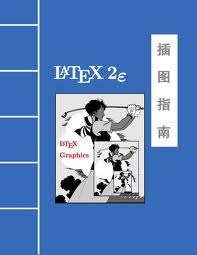
\includegraphics[width=0.5\textwidth]{latex_figure.jpeg}
\caption{\LaTeX{}插图指南}
\label{fig:1}
\end{figure}
通过图\ref{fig:1},我们可以得出\ldots

\subsubsection{参考文献}

BibTeX 模板格式分为好几类:article\cite{1:article}, book\cite{2:book}, misc\cite{3:misc}等等 

\section{数学公式}

\subsection{综述}

\subsubsection{行间式样}

和的平方:$c^{2}=a^{2}+b^{2}$

心型:\begin{math}\heartsuit\end{math}

$\lim_{n \to \infty}\sum_{k=1}^n \frac{1}{k^2} = \frac{\pi^2}{6}$

\subsubsection{显示式样}

求$a$与$b$的和:
\begin{displaymath}a+b=c\end{displaymath}

和的平方:\[c^{2}=a^{2}+b^{2}\]

\begin{displaymath}
\lim_{n \to \infty}
\sum_{k=1}^n \frac{1}{k^2}
= \frac{\pi^2}{6}
\end{displaymath}

\subsubsection{公式编号}

\begin{equation} \label{eq:eps}
\epsilon > 0
\end{equation}
从公式(\ref{eq:eps}), 我们得出\ldots

\subsection{数学模式的群组}

\begin{equation}
a^x+y \neq a^{x+y}
\end{equation}

\subsection{数学公式的基本元素}

\begin{description}
\item[希腊字母]
$\alpha, \beta, \gamma, \Gamma, \Delta, \lambda, \xi, \pi, \mu, \Phi, \Omega$

\item[指数和下标]$a_{1}$, $e^{x^2}\neq {e^x}^2$

\item[平方根] $\sqrt{x}$, $\sqrt[3]{2}$ 

\item[水平线]$\overline{m+n}$, $\underline{m+n}$

\item[水平括号] $\underbrace{a+b+\cdots+z}_{26}$

\item[导数]$y=x^{2}\qquad y’=2x\qquad y’’=2$

\item[乘号]$x_{1}\cdot x_{2}$

\item[log等类的函数名通常用直立字体]
\begin{flushleft}$\arccos, \cos, \csc, \exp, \ker, \limsup,\arcsin, \cosh, \deg, \gcd, \lg, \ln, \arctan$\\$ \cot \det, \hom, \lim, \log,
\arg, \coth, \dim, \inf, \liminf, \max, \sinh, \sup, \tan$\\$ \tanh, \min, \Pr,
\sec, \sin$ 如极限:$\lim_{x \rightarrow 0}\frac{\sin x}{x}=1$
\end{flushleft}

\item[取模函数]$a\bmod b$, $x\equiv a \pmod{b}$

\item[分式]$1\frac{1}{2}$, $\frac{x^2}{k+1}$, $1/2$

\item[二项式系数]$\binom{n}{k},\mathrm{C}_n^k$

\item[符号堆积]$\stackrel{!}{=}$

\item[积分号,累加,累乘]$\int_{0}^{\frac{\pi}{2}} \qquad \sum_{i=1}^{n} \qquad \prod_\epsilon$

\item[括号]
\begin{itemize}
\item 自动调整括号尺寸 
\begin{displaymath}
1 + \left( \frac{1}{ 1-x^{2} }
\right) ^3
\end{displaymath}
\item 指定括号尺寸
$\big(\Big(\bigg(\Bigg($\quad$\big\}\Big\}\bigg\}\Bigg\}$\quad
$\big\|\Big\|\bigg\|\Bigg\|$
\end{itemize}

\item[竖直点列,对角线点列]$\vdots\quad \ddots$
\end{description}

\subsection{垂直取齐}

\begin{displaymath}
\mathbf{X} =
\left( \begin{array}{ccc}
x_{11} & x_{12} & \ldots \\
x_{21} & x_{22} & \ldots \\
\vdots & \vdots & \ddots
\end{array} \right)
\end{displaymath}

\begin{displaymath}
y = \left\{ \begin{array}{ll}
a & \textrm{if $d>c$}\\
b+x & \textrm{in the morning}\\
l & \textrm{all day long}
\end{array} \right.
\end{displaymath}

\begin{displaymath}
\left(\begin{array}{c|c}
1 & 2 \\
\hline
3 & 4
\end{array}\right)
\end{displaymath}

等号取齐:
\begin{eqnarray}
f(x) & = & \cos x
\\
f’(x) & = & -\sin x
\\
\int_{0}^{x} f(y)dy &
= & \sin x
\end{eqnarray}

长等式指定在哪断和如何缩进:
{\setlength\arraycolsep{2pt}
\begin{eqnarray}
\sin x & = & x -\frac{x^{3}}{3!}
+\frac{x^{5}}{5!}-{}
\nonumber\\
&& {}-\frac{x^{7}}{7!}+{}\cdots
\end{eqnarray}}

\begin{eqnarray}
\lefteqn{ \cos x = 1
-\frac{x^{2}}{2!} +{} }
\nonumber\\
& & {}+\frac{x^{4}}{4!}
-\frac{x^{6}}{6!}+{}\cdots
\end{eqnarray}

\subsection{虚位}

${}^{12}_{\phantom{1}6}\textrm{C} \qquad {}^{12}_{6}\textrm{C} $

$\Gamma_{ij}^{\phantom{ij}k} \qquad \Gamma_{ij}^{k} $ 

\subsection{定理、定律}

\newtheorem{law}{Law} %定理
\begin{law}\label{law:t} 
This is my interesting theorem.
\end{law}
通过定理\ref{law:t},我们得出\ldots

\begin{proof}
\[E=mc^2\]
\end{proof}

\subsection{粗体符号}

\begin{displaymath}
\mu, M \qquad
\boldsymbol{\mu}, \boldsymbol{M}
\end{displaymath}

\section{代码高亮}

\subsection{Matlab}

\lstinputlisting{matlab_code.m} %插入Matlab代码({}中为代码地址)

\subsection{python}

\begin{lstlisting}
for i = 1:3
\end{lstlisting}

\begin{python}
#!/usr/local/bin/python
print "Hello World"
os.system("""
VAR=even;
sed -i "s/$VAR/odd/" testfile;
for i in `cat testfile` ;
do echo $i; done;
echo "now the tr command is removing the vowels";
cat testfile |tr 'aeiou' ' '
""") 
\end{python}

\subsection{bash}

\begin{bash}
#!/bin/bash
if [ $# == 1 ]; then
    echo -ne "Deleting FILES including [$1] in the CURRENT directory ...\n\n"
    for i in $(tree -a -f -i | grep "$1")
    do
      echo -ne "Deleting $i\n"
      rm -f $i
    done
elif [ $# == 2 ]; then
    echo -ne "Deleting FILES including [$1] in [$2] directory ...\n"
    for i in $(tree -a -f -i $2 |grep "$1")
    do
      echo -ne "Deleting $i\n"
      rm -f $i
    done    
else
    echo -ne "Arguments Error.\n"
    echo -ne "Usage:\n"
    echo -ne "\t$0 STRING\n"
    echo -ne "\t$0 STRING DIRECTORY\n"
fi
cd ~/
\end{bash}

\subsection{plain}

\begin{plaintext}
user = zhenghaiyong
email = zhenghaiyong@gmail.com
\end{plaintext}

% references
\bibliographystyle{plain}

\bibliography{template} %参考文献




\end{document}
